\section{MoE at Scale}
\begin{frame}{}
    \LARGE \textbf{MoE at Scale: Load Balancing, Switch Transformers, and Parallelism}
\end{frame}

\begin{frame}{Notable MoE Papers}
    \begin{itemize}
        \item Switch Transformer (Fedus et al., 2021): Efficient routing and scaling.
        \item GShard (Lepikhin et al., 2020): Large-scale MoE for multilingual translation.
        \item M6, GLaM, and recent GPT-MoE variants: Further advances in scaling and performance.
    \end{itemize}
\end{frame}

\begin{frame}[allowframebreaks]{Load Balancing in MoEs}
    \textbf{Problem:} Without intervention, the gating network tends to route most tokens to a few experts, leading to inefficient training and poor expert utilization.

    \begin{itemize}
        \item \textbf{Expert Overload:} Popular experts receive more tokens, train faster, and become even more favored.
        \item \textbf{Underutilization:} Other experts receive few or no tokens, limiting their contribution.
    \end{itemize}

    \textbf{Solution:} Introduce an auxiliary loss to encourage balanced token distribution across experts.

    \begin{itemize}
        \item \textbf{Auxiliary Loss:} Penalizes uneven assignment of tokens, pushing the gating network to distribute tokens more uniformly.
        \item \textbf{Expert Capacity:} Each expert is assigned a maximum number of tokens it can process (capacity). Excess tokens are dropped or rerouted.
        \item \textbf{Implementation:} In transformer-based MoEs, this is often controlled via an \texttt{aux\_loss} parameter.
    \end{itemize}

    \framebreak

    \textbf{Auxiliary Loss (Switch Transformer, Eq.~4):} for a batch $\mathcal{B}$ of $T$ tokens routed over $N$ experts,
    \[
        L_{\text{aux}} = \alpha \cdot N \cdot \sum_{i=1}^{N} f_i P_i,
        \qquad
        f_i = \frac{1}{T}\sum_{x \in \mathcal{B}} \mathbf{1}\{\arg\max p(x) = i\},
        \qquad
        P_i = \frac{1}{T}\sum_{x \in \mathcal{B}} p_i(x)
    \]

    \begin{itemize}
        \item $f_i$ is the fraction of tokens \emph{dispatched} to expert $i$; $P_i$ is the fraction of router \emph{probability} given to expert $i$; $p_i(x)$ is the router's softmax score.
        \item $f_i$ comes from an $\arg\max$, so it carries no gradient. The router learns through $P_i$, which is differentiable: the loss pushes probability mass away from experts that are already receiving many tokens.
        \item The dot product $\sum_i f_i P_i$ is minimised when both vectors are uniform, which is exactly an even split of tokens across experts.
        \item The factor $N$ keeps the loss on the same scale as the number of experts changes; Fedus et al.\ use $\alpha = 10^{-2}$.
    \end{itemize}

\framebreak

    \textbf{Benefits:}
    \begin{itemize}
        \item Ensures all experts are trained and utilized.
        \item Improves model efficiency and generalization.
        \item Prevents bottlenecks and overload in popular experts.
    \end{itemize}
\end{frame}

\begin{frame}[allowframebreaks]{MoEs and Transformers}
    \textbf{Transformers and Scaling:} Transformers demonstrate that increasing the number of parameters improves performance. Google’s GShard project explored scaling transformers beyond 600 billion parameters using MoE layers.

    \begin{itemize}
        \item \textbf{GShard Approach:} Replaces every other feed-forward (FFN) layer with an MoE layer using top-2 gating in both encoder and decoder.
        \item \textbf{Distributed Training:} MoE layers are shared across devices, while other layers are replicated, enabling efficient large-scale computation.
    \end{itemize}

    \begin{figure}
        \centering
        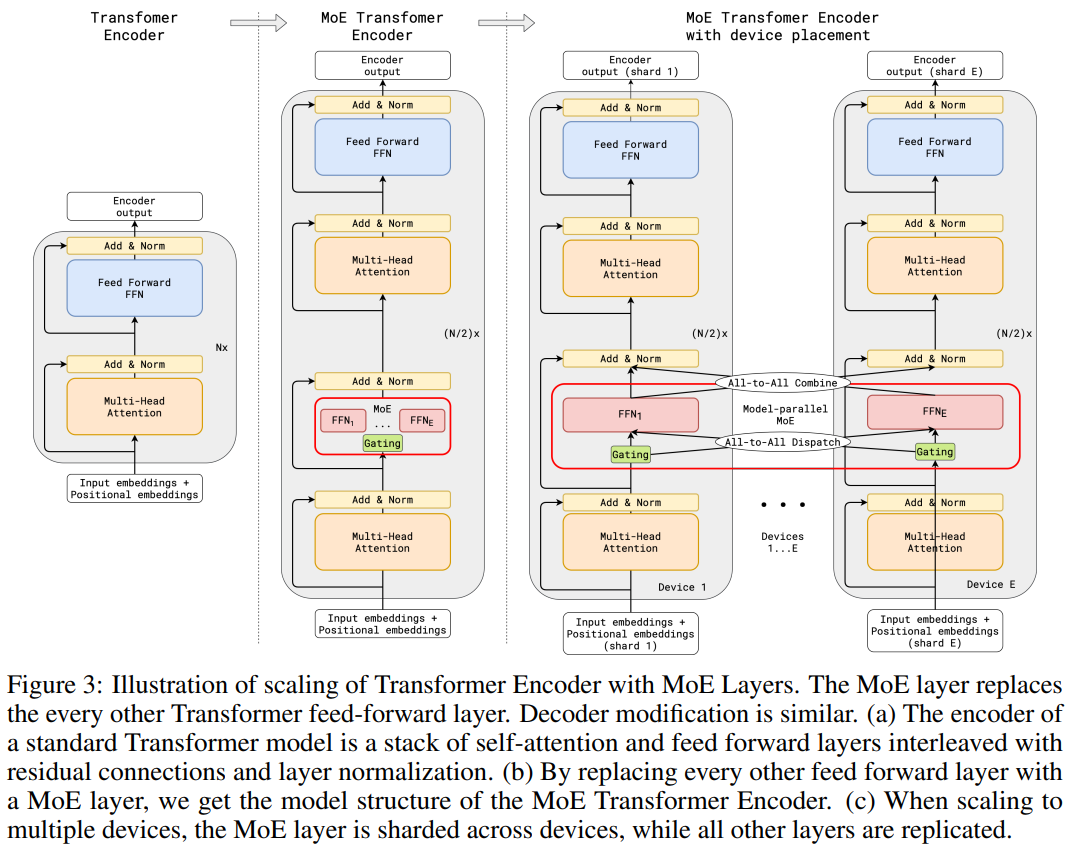
\includegraphics[width=\textwidth,height=0.78\textheight,keepaspectratio]{images/lrm+moe/gshard.png}
        \caption*{\scriptsize Source: \href{https://arxiv.org/pdf/2006.16668}{Lepikhin et al. (2020)}, Fig.~3.}
    \end{figure}

\framebreak

    \textbf{Load Balancing and Efficiency:}
    \begin{itemize}
        \item \textbf{Random Routing:} In top-2 gating, the top expert is always selected, while the second expert is chosen probabilistically based on its gating weight.
        \item \textbf{Expert Capacity:} Each expert has a maximum token capacity. Overflow tokens are either sent via residual connections or dropped, ensuring static tensor shapes and balanced computation.
    \end{itemize}

    \textbf{Why Expert Capacity?}
    \begin{itemize}
        \item Tensor shapes must be fixed at compile time, but token distribution to experts is dynamic. Capacity factors ensure compatibility and efficiency.
    \end{itemize}

\framebreak

    \textbf{Inference Efficiency:}
    \begin{itemize}
        \item During inference, only a subset of experts is activated per input.
        \item Shared computations (e.g., self-attention) are applied to all tokens, so the effective compute is much lower than the total parameter count.
        \item Example: Mixtral 8x7B has about 47B total parameters but activates only about 13B per token with top-2 gating, so its inference compute is close to that of a 13B dense model.
    \end{itemize}
\end{frame}

\begin{frame}[allowframebreaks]{Switch Transformers}
    \textbf{Switch Transformers:} Address training and fine-tuning instabilities in MoEs by simplifying routing and improving efficiency. The authors released a 1.6T parameter MoE model with 2048 experts on Hugging Face, achieving a 4x pre-train speed-up over T5-XXL.

    \begin{itemize}
        \item \textbf{Switch Transformer Layer:} Replaces FFN layers with MoE layers, but routes each token to a single expert (single-expert strategy), reducing router computation and communication costs while preserving quality.
        \item \textbf{Expert Capacity:} Defined as
        \[
            \text{Expert Capacity} = \left(\frac{\text{tokens per batch}}{\text{number of experts}}\right) \times \text{capacity factor}
        \]
        \item Low capacity factors (1--1.25) are effective, balancing efficiency and communication overhead.
        \item \textbf{Load Balancing Loss:} Simplified auxiliary loss encourages uniform routing and is weighted by a hyperparameter.
        \item \textbf{Selective Precision:} Experts are trained in bfloat16, while routing uses full precision to avoid instability. This reduces communication and computation costs without degrading quality.
    \end{itemize}

\framebreak

    \begin{figure}
        \centering
        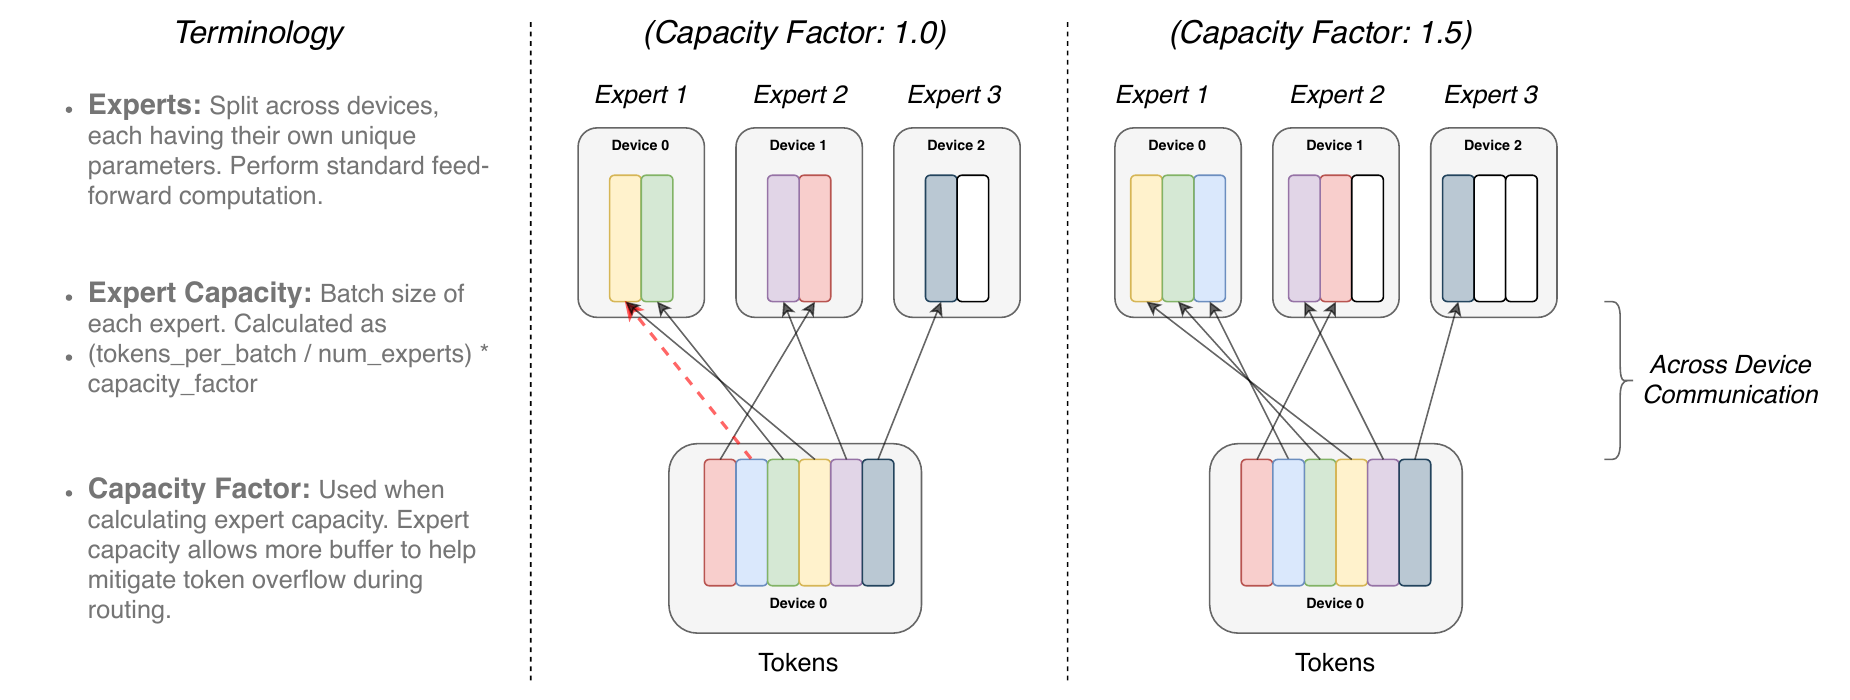
\includegraphics[width=\textwidth,height=0.72\textheight,keepaspectratio]{images/lrm+moe/switch_token_routing_capacity.png}
        \caption*{\scriptsize Each expert processes a fixed batch of (tokens per batch / experts) $\times$ capacity factor. At a capacity factor of 1.0 an overloaded expert overflows and the extra token is dropped (dashed red); at 1.5 nothing is dropped, at the cost of padded empty slots (white). Source: \href{https://arxiv.org/pdf/2101.03961}{Fedus et al. (2021)}, Fig.~3.}
    \end{figure}

\framebreak

    \textbf{Architecture:}
    \begin{itemize}
        \item Encoder-decoder setup, similar to T5 but with MoE layers.
        \item Fine-tuning and summarization tasks are supported.
    \end{itemize}

    \textbf{GLaM and Scaling:}
    \begin{itemize}
        \item GLaM explores scaling MoEs further, matching GPT-3 quality with 1/3 the energy.
        \item Uses decoder-only models, top-2 routing, and larger capacity factors.
        \item Capacity factor can be adjusted during training and inference to control compute and efficiency.
    \end{itemize}
\end{frame}

\begin{frame}[allowframebreaks]{DeepSeekMoE: Fine-Grained and Shared Experts}
    \textbf{Design:} DeepSeek-V3 has 671B total parameters and activates 37B of them per token; DeepSeek-R1 is trained from it and inherits the same architecture. Every feed-forward layer except the first three is an MoE layer holding 1 shared expert and 256 routed experts, of which 8 are activated per token.

    \begin{itemize}
        \item \textbf{Fine-grained segmentation:} each expert is made smaller and more of them are activated. Splitting $N$ experts into $mN$ smaller ones and activating $mk$ instead of $k$ leaves the active parameter count unchanged, but gives far more distinct combinations of experts, so each one can specialise more narrowly.
        \item \textbf{Shared experts:} a small number of experts are always active for every token. They absorb the knowledge every token needs, which keeps that knowledge from being duplicated inside every routed expert.
    \end{itemize}

\framebreak

    \textbf{Auxiliary-loss-free load balancing:}
    \begin{itemize}
        \item An auxiliary loss balances experts, but it competes with the language-modelling objective: too large a coefficient costs quality.
        \item DeepSeek-V3 instead keeps a bias $b_i$ per expert and adds it to the affinity score when choosing the top-$k$. Overloaded experts have their bias decreased and underloaded experts increased, by a fixed step at each training step.
        \item The bias only decides \emph{which} experts are selected. The gating value that multiplies an expert's output is still computed from the original affinity score, so the forward pass is left undistorted.
        \item A sequence-wise balance loss is retained with a very small weight ($\alpha = 10^{-4}$), only to rule out extreme imbalance inside a single sequence.
    \end{itemize}
\end{frame}

\begin{frame}[allowframebreaks]{Parallelism in MoE}
    \textbf{Parallelism Overview:}
    \begin{itemize}
        \item \textbf{Data Parallelism:} Replicates model weights across all cores; data is partitioned so each core processes a different batch.
        \item \textbf{Model Parallelism:} Splits the model across cores; each core holds a part of the model, and data is replicated.
        \item \textbf{Model and Data Parallelism:} Both model and data are partitioned; different cores process different batches and hold different model segments.
        \item \textbf{Expert Parallelism:} Experts are distributed across workers. Each worker processes a different batch, and MoE layers route tokens to the appropriate expert on each worker.
    \end{itemize}

    \textbf{Expert Parallelism Details:}
    \begin{itemize}
        \item For non-MoE layers, expert parallelism acts like data parallelism.
        \item For MoE layers, tokens are dynamically routed to the worker hosting the selected expert.
        \item Enables scaling to large numbers of experts and efficient distributed training.
    \end{itemize}

    \begin{figure}
        \centering
        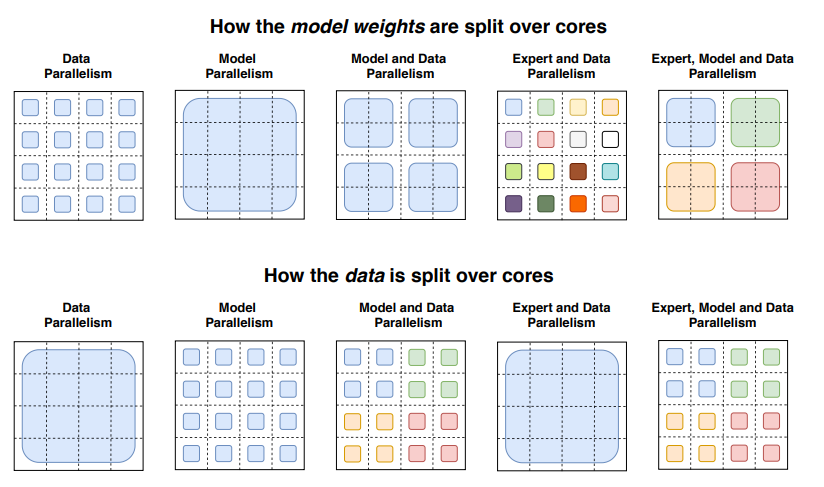
\includegraphics[height=0.6\textheight,width=1\textwidth,keepaspectratio]{images/recent-advance/moe-parallelism.png}
        \caption*{\scriptsize Each $4\times4$ grid is 16 cores; the top row shows how model weights are split across them and the bottom row how the batch of tokens is split. Source: \href{https://arxiv.org/pdf/2101.03961}{Fedus et al. (2021)}, Fig.~9.}
    \end{figure}
\end{frame}

